% Beamer Presentation: Sciara-fv2 CUDA Performance Analysis
% Author: Nhat Quang Dang
% University of Calabria
% Date: January 15, 2025

\documentclass[aspectratio=169]{beamer}

% === THEME: University of Calabria Red ===
\usetheme{Madrid}
\usecolortheme{beaver}
\definecolor{unicalred}{RGB}{180, 30, 30}
\definecolor{unicalredlight}{RGB}{220, 80, 80}
\setbeamercolor{palette primary}{bg=unicalred,fg=white}
\setbeamercolor{palette secondary}{bg=unicalredlight,fg=white}
\setbeamercolor{palette tertiary}{bg=unicalred,fg=white}
\setbeamercolor{structure}{fg=unicalred}
\setbeamercolor{title}{fg=white,bg=unicalred}  % white text on red background
\setbeamercolor{frametitle}{fg=unicalred}
\setbeamercolor{block title}{bg=unicalred,fg=white}
\setbeamercolor{block body}{bg=unicalred!10}

% === REMOVE SHADOWS ===
\setbeamertemplate{blocks}[default]  % remove block shadows
\setbeamertemplate{title page}[default]  % remove title page shadows
\setbeamertemplate{items}[default]  % remove item shadows

% === NUMBERED SECTIONS IN TOC ===
\setbeamertemplate{section in toc}[sections numbered]  % add numbers to TOC

% === PACKAGES ===
\usepackage{graphicx}
\usepackage{booktabs}
\usepackage{colortbl}  % for \rowcolor
\usepackage{tikz}
\usetikzlibrary{shapes.geometric, arrows, positioning, calc}
\usepackage{pgfplots}
\pgfplotsset{compat=1.17}
\usepackage{xcolor}
\usepackage{fontawesome5}

% === METADATA ===
\title[Sciara-fv2 CUDA]{CUDA Parallelization of Sciara-fv2\\Lava Flow Simulator}
\subtitle{Performance Analysis and Optimization}
\author[N.Q. Dang]{Nhat Quang Dang\\{\small Reg. No. 279990}}
\institute[UNICAL]{
    \includegraphics[height=1cm]{fig1.eps}\\[0.3cm]
    University of Calabria\\
    {\small\texttt{dngntq02p19z251l@studenti.unical.it}}
}
\date{January 15, 2025}

% === DOCUMENT ===
\begin{document}

% ------ TITLE SLIDE ------
\begin{frame}
    \titlepage
\end{frame}

% ------ OUTLINE ------
\begin{frame}{Outline}
    \tableofcontents
\end{frame}

% ============================================================================
\section{Context}
% ============================================================================

\begin{frame}{Context: Sciara-fv2 Lava Flow Simulator}
    \begin{columns}
        \begin{column}{0.55\textwidth}
            \textbf{What is Sciara-fv2?}
            \begin{itemize}
                \item Cellular Automata model for \textbf{lava flow simulation}
                \item Simulates Mt. Etna 2006 eruption
                \item Grid: 517 $\times$ 378 = \textbf{195,426 cells}
                \item Each cell: altitude, lava thickness, temperature
            \end{itemize}

            \vspace{0.5cm}
            \textbf{Challenge:}
            \begin{itemize}
                \item Moore neighborhood (9 cells stencil)
                \item Memory-intensive computation
                \item Need GPU parallelization
            \end{itemize}
        \end{column}
        \begin{column}{0.45\textwidth}
            \begin{center}
            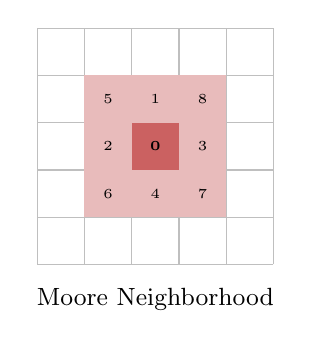
\begin{tikzpicture}[scale=0.6]
                % Grid
                \draw[step=1, gray!50] (0,0) grid (5,5);
                % Center cell
                \fill[unicalred!70] (2,2) rectangle (3,3);
                % Neighbors
                \foreach \x/\y in {1/1, 2/1, 3/1, 1/2, 3/2, 1/3, 2/3, 3/3} {
                    \fill[unicalred!30] (\x,\y) rectangle (\x+1,\y+1);
                }
                % Labels
                \node at (2.5, 2.5) {\tiny\textbf{0}};
                \node at (2.5, 3.5) {\tiny 1};
                \node at (1.5, 2.5) {\tiny 2};
                \node at (3.5, 2.5) {\tiny 3};
                \node at (2.5, 1.5) {\tiny 4};
                \node at (1.5, 3.5) {\tiny 5};
                \node at (3.5, 1.5) {\tiny 7};
                \node at (1.5, 1.5) {\tiny 6};
                \node at (3.5, 3.5) {\tiny 8};
                % Caption
                \node[below] at (2.5, -0.3) {\small Moore Neighborhood};
            \end{tikzpicture}
            \end{center}

            \vspace{0.3cm}
            \begin{block}{GPU Target}
                NVIDIA GTX 980 (Maxwell)\\
                2048 CUDA cores, 2MB L2 cache
            \end{block}
        \end{column}
    \end{columns}
\end{frame}

% ============================================================================
\section{Roadmap}
% ============================================================================

\begin{frame}{Roadmap: 5 CUDA Optimization Strategies}
    \begin{center}
    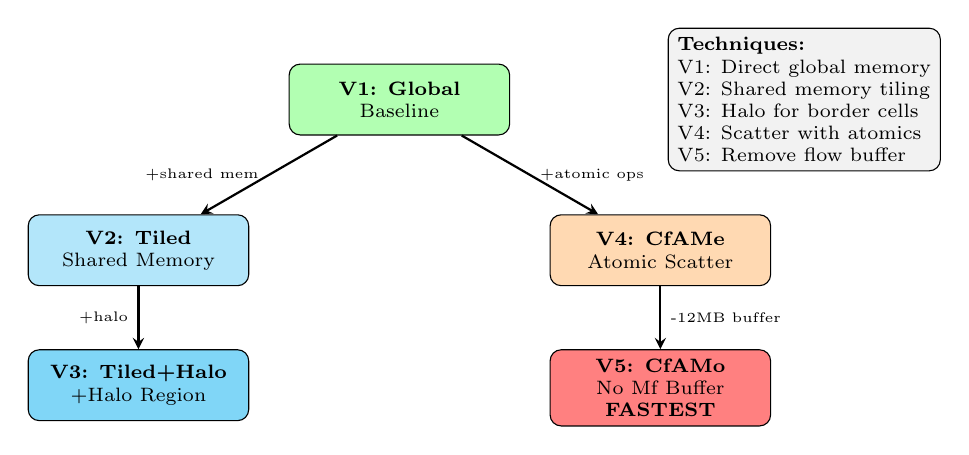
\begin{tikzpicture}[
        node distance=0.8cm,
        box/.style={rectangle, draw, rounded corners, minimum width=2.8cm, minimum height=0.9cm, align=center, font=\scriptsize},
        arrow/.style={->, thick, >=stealth}
    ]

    % Baseline
    \node[box, fill=green!30] (global) {\textbf{V1: Global}\\Baseline};

    % Branch 1: Tiled
    \node[box, fill=cyan!30, below left=1cm and 0.5cm of global] (tiled) {\textbf{V2: Tiled}\\Shared Memory};
    \node[box, fill=cyan!50, below=of tiled] (halo) {\textbf{V3: Tiled+Halo}\\+Halo Region};

    % Branch 2: Atomic
    \node[box, fill=orange!30, below right=1cm and 0.5cm of global] (cfame) {\textbf{V4: CfAMe}\\Atomic Scatter};
    \node[box, fill=red!50, below=of cfame] (cfamo) {\textbf{V5: CfAMo}\\No Mf Buffer\\\textbf{FASTEST}};

    % Arrows
    \draw[arrow] (global) -- (tiled) node[midway, left, font=\tiny] {+shared mem};
    \draw[arrow] (global) -- (cfame) node[midway, right, font=\tiny] {+atomic ops};
    \draw[arrow] (tiled) -- (halo) node[midway, left, font=\tiny] {+halo};
    \draw[arrow] (cfame) -- (cfamo) node[midway, right, font=\tiny] {-12MB buffer};

    % Legend box
    \node[draw, fill=gray!10, rounded corners, right=2cm of global, font=\scriptsize, align=left] (legend) {
        \textbf{Techniques:}\\
        V1: Direct global memory\\
        V2: Shared memory tiling\\
        V3: Halo for border cells\\
        V4: Scatter with atomics\\
        V5: Remove flow buffer
    };

    \end{tikzpicture}
    \end{center}

    \vspace{0.3cm}
    \begin{columns}
        \begin{column}{0.5\textwidth}
            \centering
            \textcolor{cyan!70!black}{\faArrowLeft\ \textbf{Tiled Branch}}\\
            {\small Reduce memory latency}
        \end{column}
        \begin{column}{0.5\textwidth}
            \centering
            \textcolor{orange!70!black}{\textbf{Atomic Branch} \faArrowRight}\\
            {\small Reduce memory footprint}
        \end{column}
    \end{columns}
\end{frame}

% ============================================================================
\section{Time Execution}
% ============================================================================

\begin{frame}{Execution Time Comparison}
    \begin{columns}
        \begin{column}{0.55\textwidth}
            \begin{center}
                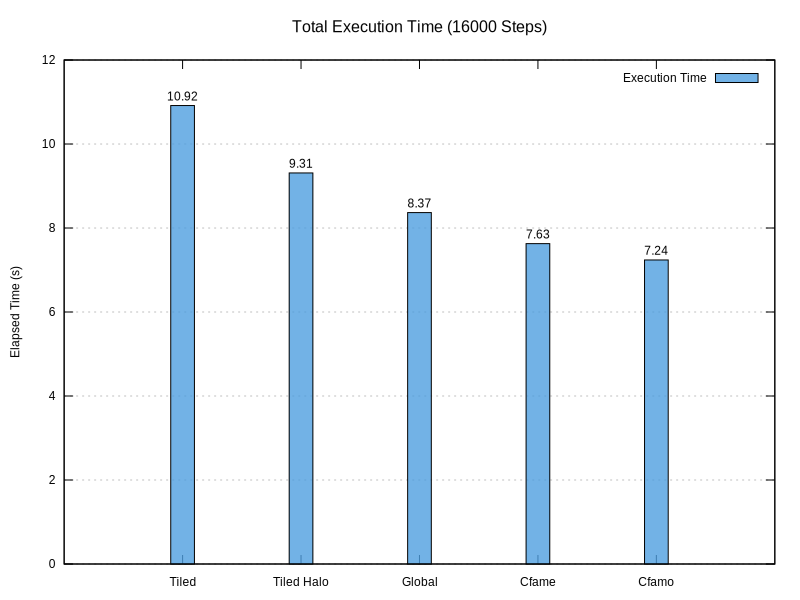
\includegraphics[width=\textwidth]{profiling_results/histogram_times.png}
            \end{center}
        \end{column}
        \begin{column}{0.45\textwidth}
            \begin{table}
                \centering
                \scriptsize
                \begin{tabular}{@{}lcc@{}}
                    \toprule
                    \textbf{Version} & \textbf{Time (s)} & \textbf{Speedup} \\
                    \midrule
                    CfAMe & 24.69 & 0.88$\times$ \\
                    Tiled+Halo & 23.33 & 0.93$\times$ \\
                    Global & 21.60 & 1.00$\times$ \\
                    Tiled & 20.14 & 1.07$\times$ \\
                    \rowcolor{unicalred!20}
                    \textbf{CfAMo} & \textbf{19.74} & \textbf{1.09$\times$} \\
                    \bottomrule
                \end{tabular}
            \end{table}

            \vspace{0.3cm}
            \begin{alertblock}{Key Finding}
                \textbf{CfAMo is fastest} despite lower occupancy!\\[0.2cm]
                {\small Eliminating 12MB flow buffer improves cache efficiency.}
            \end{alertblock}
        \end{column}
    \end{columns}
\end{frame}

% ============================================================================
\section{Roofline Model}
% ============================================================================

\begin{frame}{Roofline Analysis}
    \begin{columns}
        \begin{column}{0.6\textwidth}
            \begin{center}
                \includegraphics[width=\textwidth]{profiling_results/roofline_fp64.png}
            \end{center}
        \end{column}
        \begin{column}{0.4\textwidth}
            \begin{block}{Observations}
                \begin{itemize}
                    \item All versions: \textbf{AI $<$ 0.05}
                    \item Ridge point: \textbf{0.694}
                    \item All are \textbf{memory-bound}
                \end{itemize}
            \end{block}

            \vspace{0.3cm}
            \begin{table}
                \centering
                \scriptsize
                \begin{tabular}{@{}lc@{}}
                    \toprule
                    \textbf{Version} & \textbf{AI} \\
                    \midrule
                    Global & 0.043 \\
                    Tiled & 0.046 \\
                    Tiled+Halo & 0.048 \\
                    CfAMe & 0.020 \\
                    CfAMo & 0.021 \\
                    \bottomrule
                \end{tabular}
            \end{table}

            \vspace{0.2cm}
            {\footnotesize\textit{Low AI = stencil access pattern\\(9 neighbors $\times$ 3 substates)}}
        \end{column}
    \end{columns}
\end{frame}

% ============================================================================
\section{GPU Occupancy}
% ============================================================================

\begin{frame}{GPU Occupancy Analysis}
    \begin{columns}
        \begin{column}{0.55\textwidth}
            \begin{center}
                \includegraphics[width=\textwidth]{profiling_results/occupancy.png}
            \end{center}
        \end{column}
        \begin{column}{0.45\textwidth}
            \begin{table}
                \centering
                \scriptsize
                \begin{tabular}{@{}lc@{}}
                    \toprule
                    \textbf{Version} & \textbf{Occupancy} \\
                    \midrule
                    Global & 55.1\% \\
                    Tiled & 58.7\% \\
                    \rowcolor{cyan!20}
                    Tiled+Halo & \textbf{62.7\%} \\
                    CfAMe & 58.6\% \\
                    CfAMo & 58.6\% \\
                    \bottomrule
                \end{tabular}
            \end{table}

            \vspace{0.3cm}
            \begin{alertblock}{Important Insight}
                \textbf{High occupancy $\neq$ Fast!}\\[0.2cm]
                Tiled+Halo has highest occupancy (62.7\%) but is \textbf{slower} than Global.\\[0.2cm]
                {\small \texttt{\_\_syncthreads()} overhead exceeds shared memory benefits.}
            \end{alertblock}
        \end{column}
    \end{columns}
\end{frame}

% ============================================================================
\section{FLOP Count}
% ============================================================================

\begin{frame}{FLOP Count Comparison}
    \begin{columns}
        \begin{column}{0.5\textwidth}
            \begin{center}
            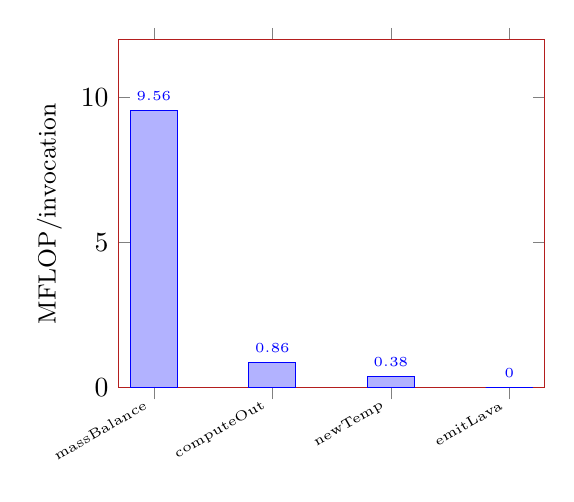
\begin{tikzpicture}
                \begin{axis}[
                    ybar,
                    width=7cm,
                    height=6cm,
                    ylabel={MFLOP/invocation},
                    ylabel style={font=\small},
                    symbolic x coords={massBalance, computeOut, newTemp, emitLava},
                    xtick=data,
                    xticklabel style={rotate=30, anchor=east, font=\tiny},
                    ymin=0,
                    ymax=12,
                    bar width=0.6cm,
                    nodes near coords,
                    nodes near coords style={font=\tiny, above},
                    every node near coord/.append style={rotate=0},
                    fill=unicalred!70,
                    draw=unicalred,
                ]
                \addplot coordinates {
                    (massBalance, 9.56)
                    (computeOut, 0.86)
                    (newTemp, 0.38)
                    (emitLava, 0.00)
                };
                \end{axis}
            \end{tikzpicture}
            \end{center}
        \end{column}
        \begin{column}{0.5\textwidth}
            \begin{table}
                \centering
                \scriptsize
                \begin{tabular}{@{}lrr@{}}
                    \toprule
                    \textbf{Kernel} & \textbf{FLOPs} & \textbf{Time\%} \\
                    \midrule
                    \rowcolor{unicalred!20}
                    massBalance & 9.56M & 27.7\% \\
                    computeOutflows & 0.86M & 24.0\% \\
                    newTemp & 0.38M & 10.5\% \\
                    emitLava & 2 & 3.2\% \\
                    \midrule
                    DtoD copies & -- & \textbf{34.7\%} \\
                    \bottomrule
                \end{tabular}
            \end{table}

            \vspace{0.3cm}
            \begin{block}{Bottleneck Analysis}
                \begin{itemize}
                    \item \textbf{34.7\%} GPU time on memory copies
                    \item massBalance: most FLOPs, most time
                    \item computeOutflows: few FLOPs but memory-heavy
                \end{itemize}
            \end{block}
        \end{column}
    \end{columns}
\end{frame}

% ============================================================================
\section{Conclusions}
% ============================================================================

\begin{frame}{Conclusions \& Key Takeaways}
    \begin{columns}
        \begin{column}{0.5\textwidth}
            \begin{block}{\faCheckCircle\ Main Results}
                \begin{enumerate}
                    \item \textbf{CfAMo is fastest} (19.74s, 1.09$\times$)
                    \item All versions are \textbf{memory-bound}
                    \item \textbf{High occupancy $\neq$ performance}
                    \item Memory footprint matters more than compute optimization
                \end{enumerate}
            \end{block}

            \vspace{0.3cm}
            \begin{block}{\faLightbulb\ Why CfAMo Wins}
                \begin{itemize}
                    \item Eliminates 12MB flow buffer
                    \item Better cache utilization
                    \item Sparse lava ($<$5\% active) minimizes atomic contention
                \end{itemize}
            \end{block}
        \end{column}
        \begin{column}{0.5\textwidth}
            \begin{block}{\faChartLine\ Performance Summary}
                \begin{center}
                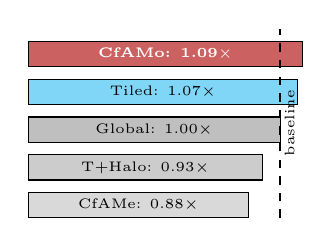
\begin{tikzpicture}[scale=0.8]
                    % Speedup bars
                    \draw[fill=gray!30] (0,0) rectangle (3.5,0.4) node[midway, font=\tiny] {CfAMe: 0.88$\times$};
                    \draw[fill=gray!40] (0,0.6) rectangle (3.72,1.0) node[midway, font=\tiny] {T+Halo: 0.93$\times$};
                    \draw[fill=gray!50] (0,1.2) rectangle (4.0,1.6) node[midway, font=\tiny] {Global: 1.00$\times$};
                    \draw[fill=cyan!50] (0,1.8) rectangle (4.28,2.2) node[midway, font=\tiny] {Tiled: 1.07$\times$};
                    \draw[fill=unicalred!70] (0,2.4) rectangle (4.36,2.8) node[midway, font=\tiny, white] {\textbf{CfAMo: 1.09$\times$}};
                    % Baseline
                    \draw[dashed, thick] (4.0,0) -- (4.0,3);
                    \node[font=\tiny, rotate=90] at (4.15,1.5) {baseline};
                \end{tikzpicture}
                \end{center}
            \end{block}

            \vspace{0.2cm}
            \begin{alertblock}{\faExclamationTriangle\ Lesson Learned}
                For small grids that fit in L2 cache, \textbf{reducing memory footprint} is more effective than shared memory tiling.
            \end{alertblock}
        \end{column}
    \end{columns}
\end{frame}

% ------ THANK YOU ------
\begin{frame}
    \begin{center}
        {\Huge\textcolor{unicalred}{Thank You!}}

        \vspace{1cm}
        {\Large Questions?}

        \vspace{1cm}
        \begin{tabular}{rl}
            \faUser & Nhat Quang Dang \\
            \faIdCard & Reg. No. 279990 \\
            \faEnvelope & \texttt{dngntq02p19z251l@studenti.unical.it} \\
            \faUniversity & University of Calabria \\
        \end{tabular}

        \vspace{0.5cm}
        {\small January 15, 2025}
    \end{center}
\end{frame}

\end{document}
